\documentclass[10pt,aspectratio=169]{beamer}

\usetheme[progressbar=frametitle]{metropolis}
\usepackage{appendixnumberbeamer}

\usepackage{booktabs}
\usepackage[scale=2]{ccicons}

\usepackage{pgfplots}
\usepgfplotslibrary{dateplot}

\usepackage{xspace}
\newcommand{\themename}{\textbf{\textsc{metropolis}}\xspace}

\usepackage[default]{lato}

\title{Protocolo de Tesis}
\subtitle{Cuantificación de incertidumbre bayesiana aproximada en problemas inversos de ODE}
% \date{\today}
\date{}
\author{César Isaí García Cornejo\\
Asesor: Dr. José Andrés Christen Gracia}
\institute{CIMAT}
% \titlegraphic{\hfill\includegraphics[height=1.5cm]{logo.pdf}}
% ////////////////////////////////////////////////////////////
% ////////////////////////////////////////////////////////////
\begin{document}

\maketitle

% \begin{frame}{Table of contents}
%   \setbeamertemplate{section in toc}[sections numbered]
%   \tableofcontents%[hideallsubsections]
% \end{frame}

\section[Introducción]{Introducción}

\begin{frame}[fragile]{Introducción}
  
  Los modelos que pretendan describir los fenómenos naturales deben ser causales, respetando orden entre causa y efecto.

  Típicamente, los modelos matemáticos precisan de condiciones iniciales o parámetros  para caracterizar la unicidad en su solución. Tales parámetros se conocen como parámetros del modelo y se interpretan como causas del fenómeno modelado. Mientras que la solución del modelo se interpreta como la predicción del fenómeno, que se asocia a los efectos.
  
\end{frame}


\begin{frame}[fragile]{Introducción}
  
  El proceso anteriormente descrito se llama problema directo o \textit{forward problem} ya que sigue la dirección de causalidad. Sin embargo, es interesante también el problema inverso, dada ciertas observaciones de las cualidades de un fenómeno (efectos), \textbf{¿es posible calcular las causas del modelo que rige el fenómeno?}

  % \begin{figure}[H] 
  %     \centering 
  %     
\includegraphics[width = 4 cm]{Figures/tambor2.png} 
  %     % \caption{}
  %     % \label{Fig. }
  % \end{figure} 

\end{frame}

\section{Antecedentes}

\begin{frame}[fragile]{Sistema físico}

  \textbf{Estudio de un sistema físico:}
  \begin{figure}[H] 
      \centering 
      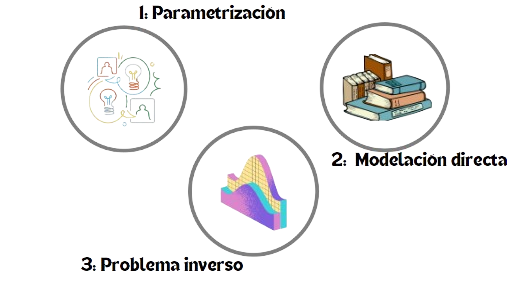
\includegraphics[width = 10 cm]{Figures/Modelos.png} 
      % \caption{}
      % \label{Fig. }
  \end{figure} 
  % \begin{enumerate}
  %     \item Parametrización del sistema: descubrimiento del conjunto mínimo de parámetros del modelo cuyos valores caracterizan completamente el sistema.
  %     \item Modelación directa (forward modeling): Descubrimiento de las leyes físicas que nos permiten hacer predicciones, dado valores de parámetros del modelo, de mediciones en observables físicas.
  %     \item Modelación inversa: Usar las mediciones de las observables físicas para inferir los valores de los parámetros del modelo.
  % \end{enumerate}

  % Los experimentos sugieren teorías físicas, y las teorías físicas predicen los resultados de los experimentos. La comparación entre la predicción y las observaciones son evidencia de la factibilidad de la teoría.
\end{frame}

\begin{frame}[fragile]{Forward map}
  
  \textbf{El problema directo:}
  
  Predecir los valores de las observables físicos $\mathbf{d}$ que corresponde a un modelo $\boldsymbol{\theta}$
  \begin{align*}
      \boldsymbol{\theta} \:\:\:\:\: \mapsto \:\:\:\:\: \mathbf{d} = \mathbf{F(\boldsymbol{\theta})}
  \end{align*}


  \vspace*{1 cm}

  Incertidumbre de las mediciones e imperfecciones del modelo \cite{tarantola2005inverse}. 

\end{frame}


\begin{frame}{Ejemplos}
  \begin{columns}[T,onlytextwidth]
    \column{0.5\textwidth}

    
    \begin{alertblock}{Resorte sujeto a fricción}
      Sea $x(t)$ la posición
      \begin{align*}
        m\ddot{x} = -kx + b \dot{x}
      \end{align*}
    \end{alertblock}
    
    \begin{block}{Caída sujeto a fricción}
      Sea $x(t)$ la posición
      \begin{align*}
        m\ddot{x} = g - b \dot{x}
      \end{align*}
          % $x(0) = \dot{x(0)} = 0$.
    \end{block}

      \begin{alertblock}{Crecimiento poblacional}
        Sea $P(t)$ el tamaño de población
        \begin{align*}
          \frac{dP}{dt} = r P \left(1 - \frac{P}{K}\right) 
        \end{align*}
      \end{alertblock}

    \column{0.5\textwidth}

      \metroset{block=fill}

      \begin{alertblock}{Forward map}
        $\theta = (k,b)  \:\:\: \mapsto \:\:\: F(\theta) = x(t)$
      \end{alertblock}
      
      \vspace*{1 cm}
      
      \begin{block}{Forward map}
        $\theta = (g,b)  \:\:\: \mapsto \:\:\: F(\theta) = x(t)$
      \end{block}

      \vspace*{1 cm}

      \begin{alertblock}{Forward map}
        $\theta = (r,K)  \:\:\: \mapsto \:\:\: F(\theta) = P(t)$
      \end{alertblock}

  \end{columns}
\end{frame}

\begin{frame}[fragile]{Estadística bayesiana}
  
  La distribución posterior 
  \begin{align*}
      \pi(\theta|x^n) &\propto \mathcal{L}(\theta|x^n) \pi(\theta)
  \end{align*}
  

\begin{figure}[H] 
    \centering 
    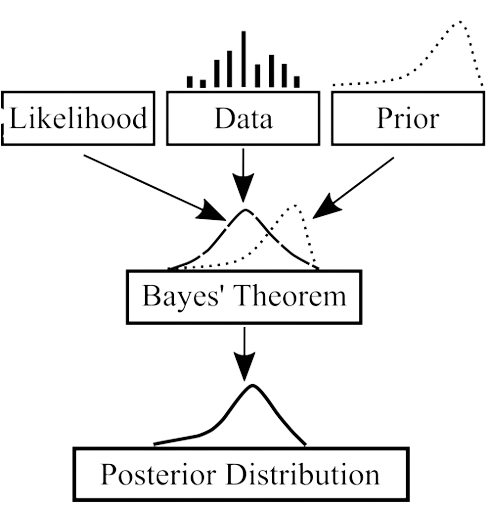
\includegraphics[width = 5.50 cm]{Figures/bayes1.png} 
    % \caption{}
    % \label{Fig. }
\end{figure} 




\end{frame}

\begin{frame}[fragile]{Incertidumbre en los errores}
  Procedimiento:
  \begin{itemize}
    \item 
    \textbf{Observaciones:} $(x_1, t_1), (x_2,t_2), \cdots, (x_n, t_n)$ 
    \item 
    Cuantificar el error mediante la relación
    \begin{align*}
        x_i = F_\theta (t_i) + \varepsilon_i, \:\:\:\:\: i = 1,...,n
    \end{align*}
    \item Un supuesto convencional sobre los errores
    \begin{align*}
        \varepsilon_i \sim N(0,\sigma^2)
        \label{3.02}
    \end{align*}

  \end{itemize}

\end{frame}

\begin{frame}[fragile]{Inferencia}
  
  Distribución posterior 
  \begin{align*}
      \pi(\theta|x^n) &\propto \mathcal{L}(\theta|x^n) \pi_{\Theta}(\theta)\\
      & \left[\propto \prod_{i=1}^n \frac{1}{\sqrt{2\pi \sigma^2}} exp \left({-\frac{1}{2\sigma^2}\left(x_i - F_{\theta}(t_i)\right)^2 }\right)\right] \pi_{\Theta}(\theta) \\
      & \propto \left(\frac{1}{2\pi\sigma^2}\right)^{n/2} exp {\left(\frac{1}{2\sigma^2} \sum_{i =1}^{n}\left(x_i - F_{\theta}(t_i)\right) ^2\right) } \pi_{\Theta}(\theta)
  \end{align*}
  donde $\theta = (\theta_1, ..., \theta_m)$.
  
  \vspace{1 cm}

  \textbf{Simular por métodos Monte Carlo}
  \begin{itemize}
    \item 
    Se simula por MCMC Metropolis-Hastings \cite{robert1999monte}.
  \end{itemize}


  % Es posible simular variables aleatorias con dicha distribución y así obtener estimaciones de los parámetros del modelo.
\end{frame}




\section{Ejemplo}


\begin{frame}{Resorte sujeto a fricción}
  \begin{figure}
      \centering 
      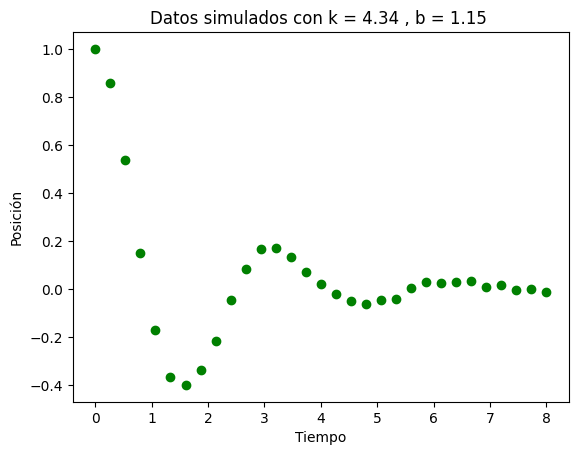
\includegraphics[width = 10cm]{Figures/0.png} 
      % \caption{}
      % \label{Fig. }
  \end{figure} 
\end{frame}

\begin{frame}
  \begin{figure}
      \centering 
      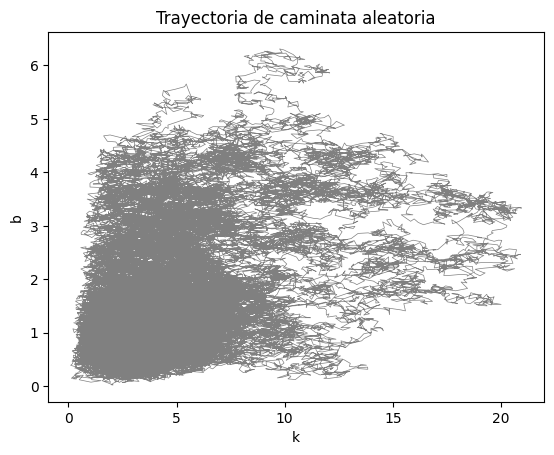
\includegraphics[width = 10 cm]{Figures/1.png} 
      % \caption{}
      % \label{Fig. }
  \end{figure} 
\end{frame}

\begin{frame}
  \begin{figure}[H] 
      \centering 
      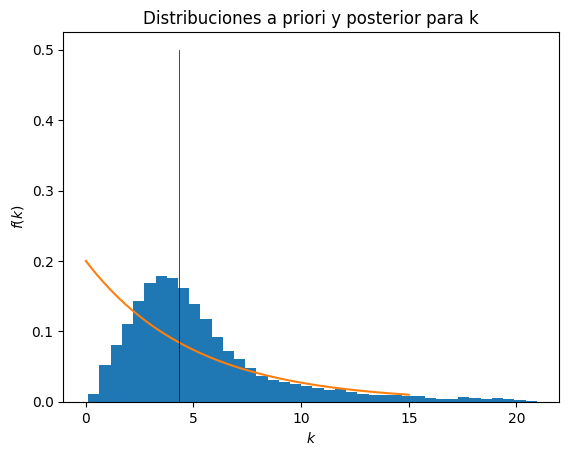
\includegraphics[width = 10 cm]{Figures/2.png} 
      % \caption{}
      % \label{Fig. }
  \end{figure} 
\end{frame}

\begin{frame}
  \begin{figure}[H] 
      \centering 
      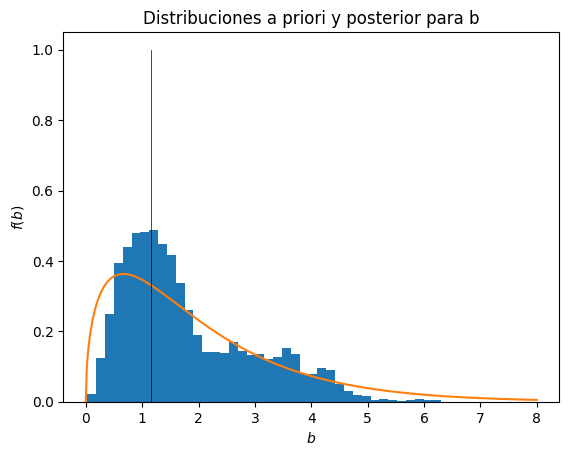
\includegraphics[width = 10 cm]{Figures/3.png} 
      % \caption{}
      % \label{Fig. }
  \end{figure} 
\end{frame}


\begin{frame}
  \begin{figure}[H] 
      \centering 
      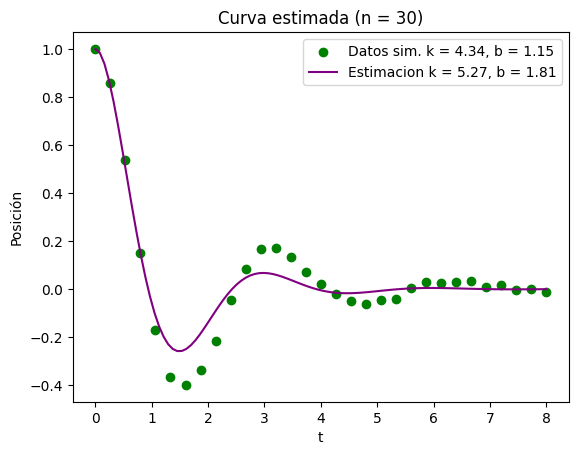
\includegraphics[width = 10 cm]{Figures/4.png} 
      % \caption{}
      % \label{Fig. }
  \end{figure} 
\end{frame}



\section{Objetivos}


\begin{frame}{Objetivos}
  A pesar de que el análisis previo nos permite obtener estimaciones bastante precisas para el problema inverso. Sin embargo, son \textbf{computacionalmente pesadas}, esto debido a que a cada paso en la cadena requiere que se solucione el problema forward, es decir, se resuelven ecuaciones diferenciales tantas veces como se deje correr la cadena. 
  \begin{itemize}
    \item 
    Se desea encontrar una especie de \textit{interpolación} para solo solucionar una cantidad pequeña de veces el problema forward y para cada punto en el espacio de parámetros se pueda aproximar la solución en función de las soluciones con parámetros cercanos.
  \end{itemize}

\end{frame}

\begin{frame}
  \begin{figure}[H] 
      \centering 
      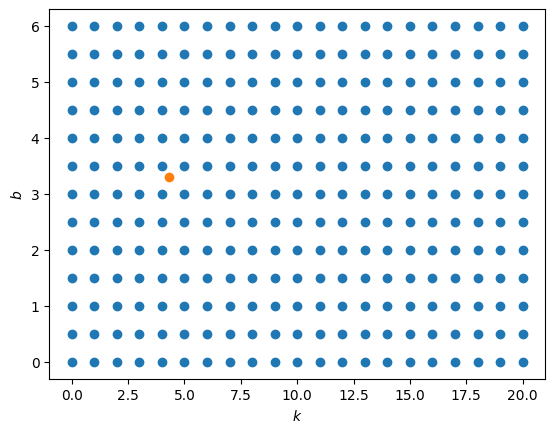
\includegraphics[width = 10 cm]{Figures/5.png} 
      % \caption{}
      % \label{Fig. }
  \end{figure} 
\end{frame}











\section{Plan de trabajo}

\begin{frame}{Plan de trabajo}
  
  \begin{figure}[H] 
      \centering 
      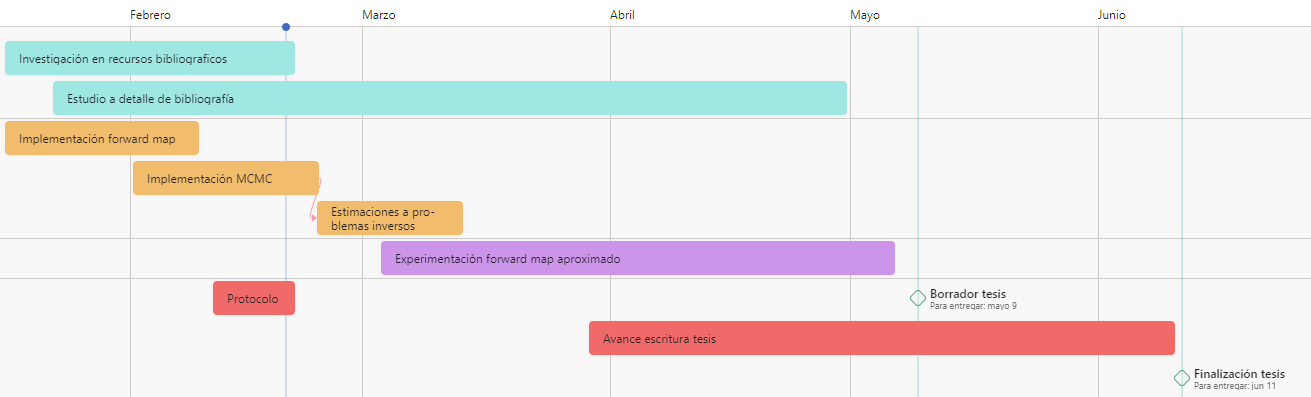
\includegraphics[width = 14 cm]{Figures/cronograma.png} 
      % \caption{}
      % \label{Fig. }
  \end{figure} 
\end{frame}



\begin{frame}{Referencias}

  \bibliography{demo}
  \bibliographystyle{abbrv}

\end{frame}



% \begin{frame}{Referencias}

  
% \end{frame}












\end{document}
